\documentclass{article}
\usepackage{fullpage}
\usepackage{pdflscape}
\usepackage{graphicx}
\usepackage{tikz}
\usetikzlibrary{trees}
\begin{document}
\begin{landscape}
\parindent=0pt
\eject\null
\vfill
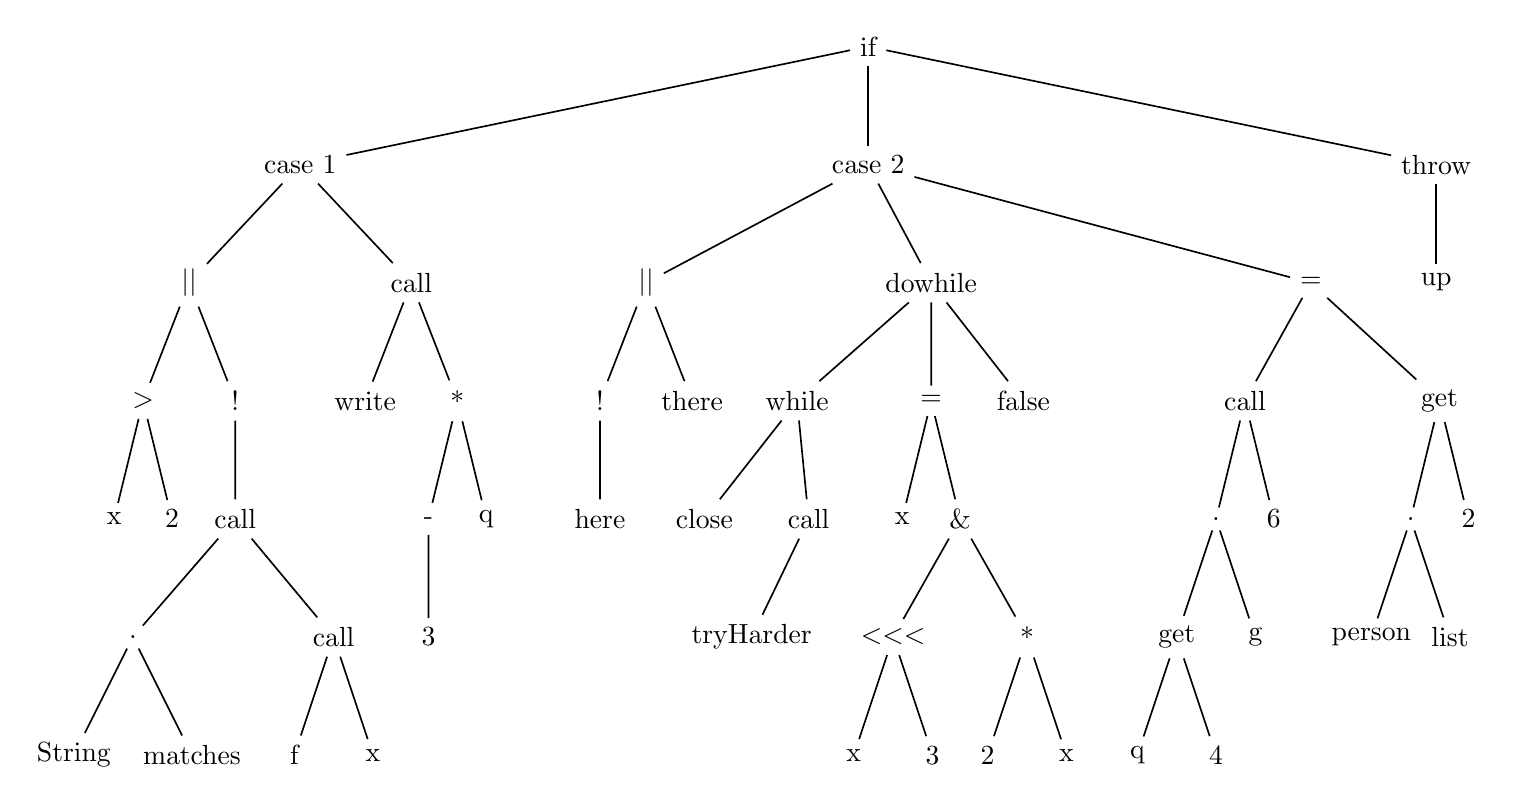
\begin{tikzpicture}[level distance=1.5cm,
  node distance=2.5cm,
  semithick,
  level 1/.style={sibling distance=7.2132cm},
  level 2/.style={sibling distance=2.8210cm},
  level 3/.style={sibling distance=1.171cm},
  level 4/.style={sibling distance=0.7342cm},
  level 5/.style={sibling distance=1cm},
  level 6/.style={sibling distance=1cm},
  level 7/.style={sibling distance=1cm}
]
\node {if}
    child {node{case 1}
        child {node{\(\vert\)\(\vert\)}
            child {node{\textgreater}
                child {node{x}}
                child {node{2}}
            }
            child {node{!}
                child {node{call}
                    child {node[xshift=-0.8cm]{.}
                        child {node[xshift=-0.25cm]{String}}
                        child {node[xshift=0.25cm]{matches}}
                    }
                    child {node[xshift=0.75cm]{call}
                        child {node{f}}
                        child {node{x}}
                    }
                }
            }
        }
        child {node{call}
            child {node{write}}
            child {node{*}
                child {node{-}
                    child {node{3}}
                }
                child {node{q}}
            }
        }
    }
    child {node{case 2}
        child {node{\(\vert\)\(\vert\)}
            child {node{!}
                child {node{here}}
            }
            child {node{there}}
        }
        child {node[xshift=0.8cm]{dowhile}
            child {node[xshift=-0.5321cm]{while}
                child {node[xshift=-0.81cm]{close}}
                child {node[xshift=-0.22cm]{call}
                    child{node[xshift=-0.723cm]{tryHarder}}
                }
            }
            child {node{=}
                child {node{x}}
                child {node{\&}
                    child {node[xshift=-0.35cm]{\textless\textless\textless}
                        child {node{x}}
                        child {node{3}}
                    }
                    child {node[xshift=0.35cm]{*}
                        child {node{2}}
                        child {node{x}}
                    }
                }
            }
            child {node{false}}
        }
        child {node[xshift=2.8cm]{=}
            child {node[xshift=-0.25cm]{call}
                child {node{.}
                    child {node{get}
                        child {node{q}}
                        child {node{4}}
                    }
                    child {node{g}}
                }
                child{node{6}}
            }
            child {node[xshift=1.05cm]{get}
                child {node{.}
                    child {node{person}}
                    child {node{list}}
                }
                child {node{2}}
            }
        }
    }
    child {node{throw}
        child {node{up}}
    };
\end{tikzpicture}
\end{landscape}
\end{document}